\chapter{Genauer Vergleich}

In diesem Kapitel werden die vorher ausgewählten Suchmaschinen genauer verglichen. Dafür werden alle vier Suchmaschinen aufgesetzt, um einen Ersteindruck zu erstellen. Da ich dieses Projekt nicht nach meiner Bachelor-Arbeit weiter betreuen kann, ist es auch wichtig zu schauen, wie leicht  es für einen neuen Administrator ist, sich in dieses System einzuarbeiten. Deshalb wird ein besonderes Augenmerk auf die Dokumentation und Oberfläche, insofern vorhanden, gelegt. Die genaueren Kriterien werden nun im Folgenden mit Erklärungen aufgeführt.

\section{Testsystem}
Das Testsystem besitzt die folgende Spezifikationen:

\begin{itemize}
    \item CPU: 4 Kerne
    \item RAM: 16 Gigabyte
    \item Festplattenspeicher: 20 GB
    \item Betriebssystem: Ubuntu 18.04.03 LTS
\end{itemize} 

Auf das System wird zudem die MariaDB Datenbank des DietrichOnline-Projektes als Datenquelle eingespielt. Zudem mussten einige Programme während der Vorbereitung des Servers durch die Administratoren aufgespielt werden. Darunter fallen Programme wie VIM oder Git. Eine genaue Liste findet sich im Anhang. Diese Programme werden als gegeben vorausgesetzt.

\section{Aufbau der Tests}

\subsection{Installation}

Im ersten Schritt wird die Installation bewertet. Dabei wird geschaut, wie einfach es ist die Software zu installieren. Existiert zum Beispiel ein Installations-Wizard? Wie viel muss manuell in den Dateien geändert werden?

\subsection{Indexierung}

Hierbei wird geschaut, wie einfach die Indexierung von den Daten aus der Datenbank ausfällt. Dabei wird auch geschaut, ob es möglich ist, Daten direkt von der Oberfläche zu indexieren und ob es möglich ist die Indexierung in einen Zeitplan zu legen.

\subsection{Oberfläche}
In diesem Schritt wird geschaut, wie übersichtlich und funktional die Oberfläche gebaut ist. Dabei geht es darum, wie viele Funktionen über die Oberfläche zu administrieren sind und ob es Komfort-Funktionen wie Responsiveness\footnote{Eine Webseite ist responsive, wenn sie für alle Endgeräte richtig skaliert und gut zu benutzen ist.} gibt.

\subsection{Dokumentation}

Im dritten Schritt wird die Dokumentation analysiert. Hier  bei wird Augenmerk auf die Übersichtlichkeit und Verständlichkeit gelegt. Da in diesem Kurztest nicht alle Bereiche der Dokumentation genau durchgelesen und daraufhin auch Testweise implementiert werden können, wird sich dabei auf die Schritte dieses Ersteindrucks bezogen.

\subsection{Absetzen einer Anfrage und Integration in PHP}

Im letzten Schritt wird eine Abfrage an das System von einem PHP-Skript abgesetzt. Dabei wird die Zeit gemessen, wie lange die Abfrage braucht um die Daten zu liefern.

Die dabei verwendete Abfrage ist die bisher am langsamsten laufenden Abfrage der DietrichOnline-Projektes. Sie ermittelt alle Lemmata vom Buchstaben S und baut alle Daten, die zur Anzeige benötigt werden zusammen \ref{img:lAdminSample}. Die Tabellen, welche für diese Ansicht gebraucht werden, sind in diesem Diagramm \ref{img:lAdminStructure} zu finden. Um genau zu sein, sind es zwei Abfragen. Die erste findet alle IDs der Lemmata und der zweite baut auf dieser Liste die Daten zusammen. Dabei werden für diesen Ersteindruck M-zu-N Beziehungen aus Zeitgründen vernachlässigt, es sei denn diese Funktionalität wird direkt mitgeliefert.

\begin{figure}
	\centering
	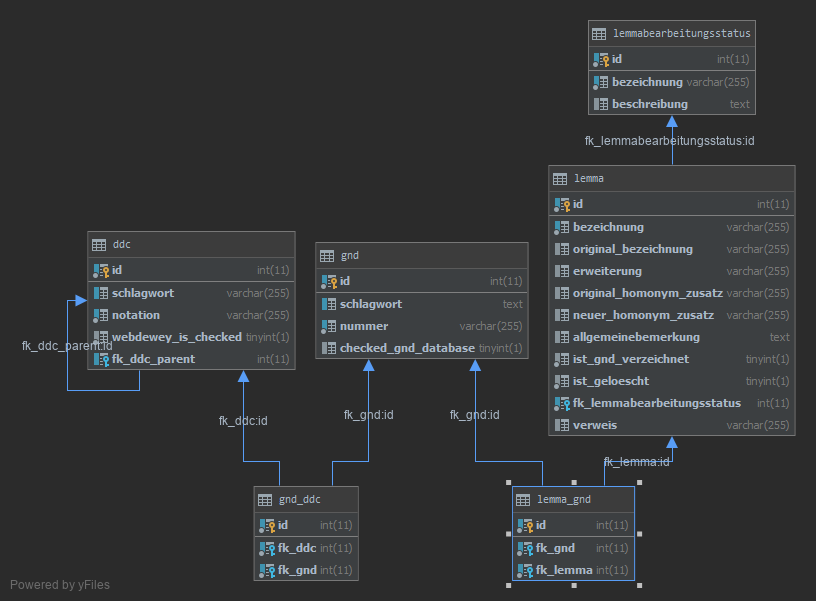
\includegraphics[width=0.8\linewidth]{images/structure_lemmaadministration.png}
	\caption{Tabellenaufbau der Lemma-Administration Übersicht.}
	\label{img:lAdminStructure}
\end{figure}

\begin{figure}
	\centering
	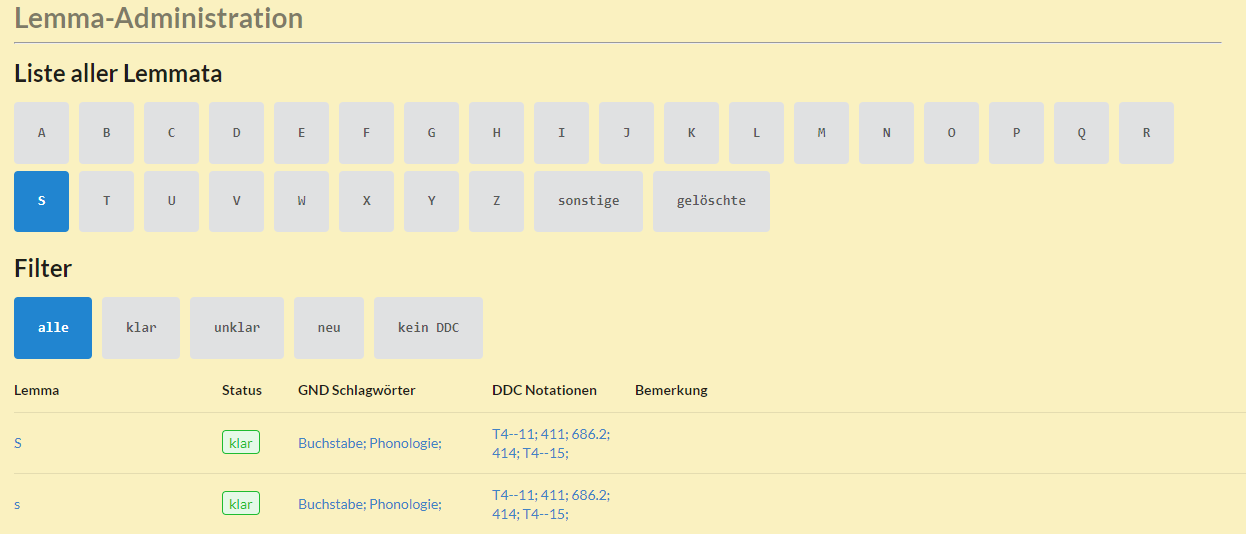
\includegraphics[width=1\linewidth]{images/lemmaadministration_sample.PNG}
	\caption{Frontend Ansicht der Lemma-Administration mit geladenen Buchstaben S (Ausschnitt).}
	\label{img:lAdminSample}
\end{figure}

\lstset{language=SQL}
\begin{lstlisting}[frame=single] 
SELECT lemma.id
FROM lemma
WHERE lemma.bezeichnung LIKE 'S%' AND lemma.ist_geloescht = 0
ORDER BY lemma.bezeichnung ASC, lemma.id ASC;
\end{lstlisting}

Im zweiten Schritt werden dann die gerade geholten ID's der Einträge mithilfe von JOIN’s für die Darstellung vorbereitet.

\lstset{language=SQL}
\begin{lstlisting}[frame=single, label={lst:sqlQuery}] 
SELECT  lemma.id, [...] #Lemma, GND und DCC-columns        
FROM lemma lemma
INNER JOIN lemmabearbeitungsstatus lemmaBStatus
ON lemma.fk_lemmabearbeitungsstatus = lemmaBStatus.id
LEFT JOIN lemma_gnd lemma_gnd_map ON lemma.id = lemma_gnd_map.fk_lemma
LEFT JOIN gnd gnd ON lemma_gnd_map.fk_gnd = gnd.id
LEFT JOIN gnd_ddc gnd_ddc_map ON gnd.id = gnd_ddc_map.fk_gnd
LEFT JOIN ddc ddc ON gnd_ddc_map.fk_ddc = ddc.id
WHERE lemma.id IN ([Array of Lemma IDs])
ORDER BY lemma.bezeichnung ASC, lemma.id ASC;

\end{lstlisting}